% Copyright (c) 2017 Peter A. Audano III
% GNU Free Documentation License Version 1.3 or later
% See the file COPYING.DOC for copying conditions.

\section{The Kestrel Process}
\label{sec.process}

Kestrel is not like other variant callers, and understanding the process is important for correctly applying it. This section discusses the process of translating sequence reads to results.


\subsection{Overview}
\label{sec.process.overview}

\begin{figure}[H]
	
	\begin{center}
		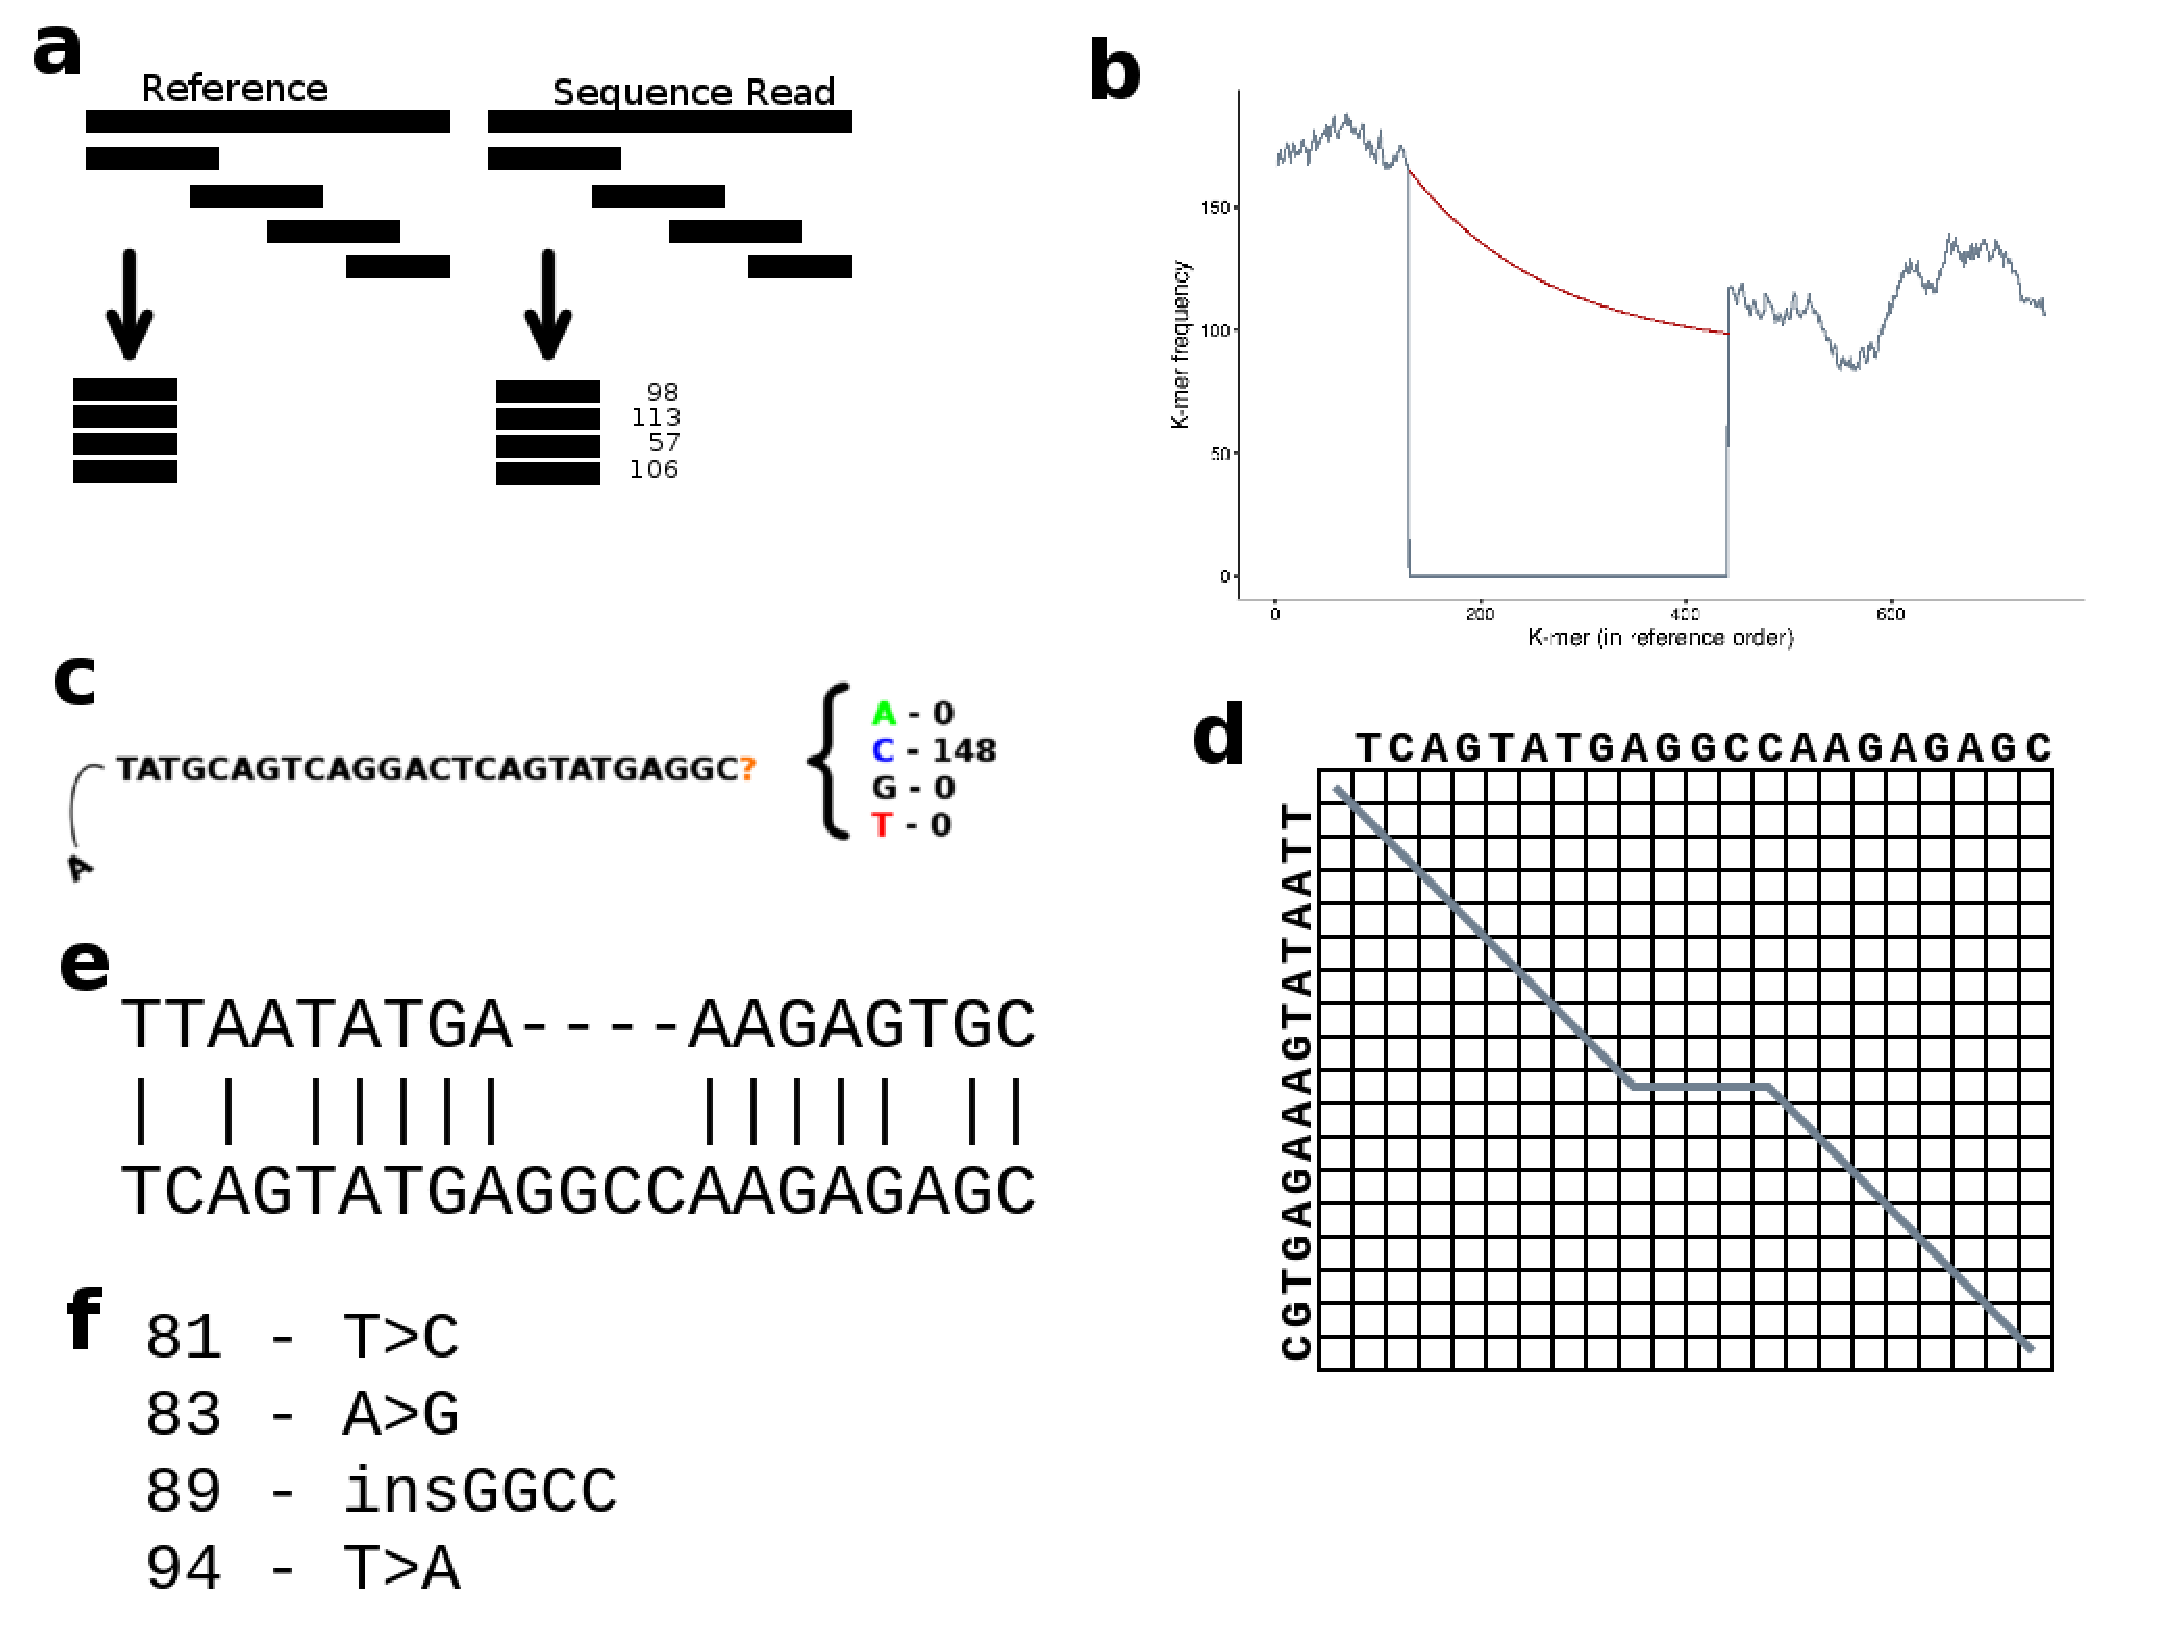
\includegraphics[width=0.75\textwidth]{img/KestrelOverview}
	\end{center}
	
	\caption{Overview of the Kestrel process from sequence data to variant call. \figpart{a} The reference sequence and the sequence reads are converted to k-mers. The k-mers of the sequence reads are counted, but the k-mers of the reference are left in order. \figpart{b} K-mer frequencies from the sequence reads (vertical axis) are assigned to the k-mers of the reference (horizontal axis). A decline and recovery of the frequencies bound an active region where one or more variants are present. \figpart{c} Starting from the left anchor k-mer (last k-mer with a high frequency), the first base is removed, each possible base is appended, and the base that recovers the k-mer frequency is appended to the haplotype. \figpart{d} A modified alignment algorithm tracks haplotype reconstruction and terminates the process when an optimal alignment is reached. \figpart{e} This algorithm yields an alignment of the reference sequence and haplotype within the active region. \figpart{f} Variant calls are extracted from the alignment.}
	
	\label{fig.arillustration}
\end{figure}

Like other variant calling approaches, Kestrel reads sequence data, compares it to a reference, and determines how the sequence data varies from the reference. The standard approach is to map the sequences to the reference and search for differences in that map. Where the sequences vary significantly from the reference, such as large insertions or dense SNPs, the read mapping step can fail. Since Kestrel does not map the sequence reads, it can recover these variations.

Instead of read mapping, sequence data is translated into a set of k-mer frequencies, and this supports the variant calls. K-mers is a short overlapping fragment of uniform length, $k$, extracted from a sequence. For example, the sequence ``ACGTAC'' in 4-mers is ``ACGT'', ``CGTA'', and ``GTAC''. These k-mers are extracted from all sequence reads, and the frequency of each unique k-mer is counted and stored in an indexed k-mer count (IKC) file on disk (\rfigpart{fig.arillustration}{a}). In real data, the k-mer size should generally between 31 and 48. Kestrel manages k-mer counting through the KAnalyze~\cite{Audano2014} application programming interface (API).

The reference sequence is also converted to k-mers of the same size, but these left in order (\rfigpart{fig.arillustration}{a}). Each reference k-mer and its reverse complement are queried from the IKC file, which gives an array of frequencies for each reference k-mer as it was found in the sample. This array is scanned for a region of k-mers where frequency drops and then recovers (\rfigpart{fig.arillustration}{b}). This defines an ``active region'' where the k-mers from the reference and the k-mers from the sample appear to be different.

The k-mer frequency database is then used as evidence to reconstruct the sequence over the active region. This reconstructed sequence is called a ``haplotype'', and each haplotype covers the whole active region. Note that more than one variant may be contained in a haplotype.

The high-frequency k-mers immediately adjacent to the low frequency k-mers in the active region are called ``anchor k-mers'', and there is one on each end of the active region. These anchor k-mers guide the haplotype reconstruction process, and they are part of the active region.

Haplotype reconstruction starts with the left anchor k-mer, which has a high frequency and is assumed to match the reference. The first base of the k-mer is removed to create a $(k - 1)$-mer. Each of the four bases are appended to the $(k - 1)$-mer in turn to see which one brings the k-mer frequency back up. This base is then added to the haplotype (\rfigpart{fig.arillustration}{c}), and this process is repeated on the new k-mer. If more than one k-mer with a high count is found during this step, the haplotype splits and multiple haplotypes are constructed.

Reconstruction must eventually cease when the haplotype is acceptable or when it cannot be an acceptable solution, so a modified Smith-waterman~\cite{Smith1981} alignment algorithm guides this step (\rfigpart{fig.arillustration}{d}). This alignment forces the haplotype and the active region to align on the left end, but it allows the haplotype to extend. When an optimal alignment is found, reconstruction is stopped.

From the alignment (\rfigpart{fig.arillustration}{e}), it is trivial to identify the variants (\rfigpart{fig.arillustration}{f}). The evidence for each variant is added from all the haplotypes that support it.


\subsection{Input}
\label{sec.process.input}

Kestrel can input sequence reads or an indexed k-mer count (IKC) file. If sequence reads are input, then k-mers are counted and output to an IKC file.

By default, all input files are part of the same sample. If multiple samples are given, then variants are called on each one independently. The command-line options in \rsec{sec.cmdline.opts.io} contain options for breaking input into discrete samples.



\subsection{Intervals}
\label{sec.process.intervals}


\subsection{K-mer Database}
\label{sec.process.kdb}


\subsection{Active Region Detection}
\label{sec.process.ardetect}


\subsection{Haplotype Reconstruction}
\label{sec.process.haplo}


\subsection{Variant Calling}
\label{sec.process.varcall}

